\documentclass{clbeamer2024}

\usepackage{minted}

\usepackage{minted}
\setminted{
	breaklines=true,
	frame=single,
	bgcolor=lightgray,
	fontsize=\small,
	escapeinside=||
}

\usepackage{xcolor}
\definecolor{bg}{rgb}{0.95, 0.95, 0.92} % Couleur gris clair

\title{
	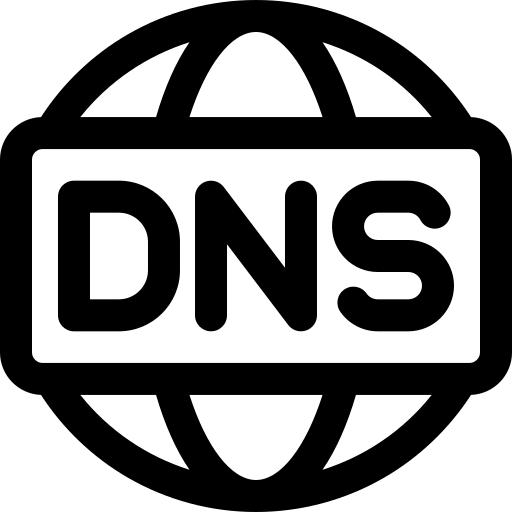
\includegraphics[width=0.8cm]{logos/dns.png} \hfill
	DNS (Domain Name System) \hfill
	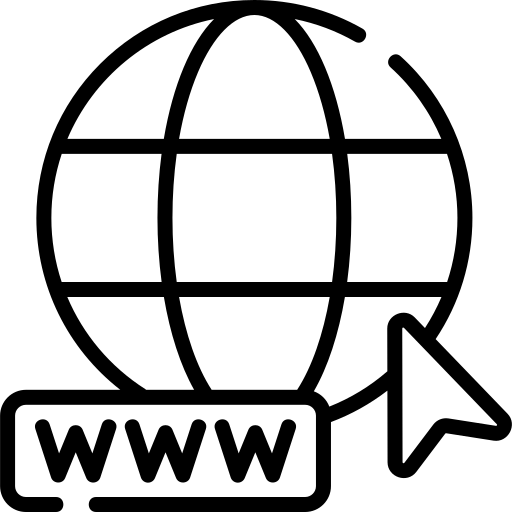
\includegraphics[width=0.95cm]{logos/browser.png}
}
\subtitle{Comprendre les bases du système de noms de domaine}
\author{Slimani Mohamed Amine}
\institute{}
\date{\today}

\begin{document}
	\setcounter{framenumber}{-1}
	\frame{\titlepage}
	
	
	
	% Sommaire
	\begin{frame}{Sommaire}
		\tableofcontents
	\end{frame}
	
	\section{Qu'est-ce que le DNS ?}
	\begin{frame}{Qu'est-ce que le DNS ?}
		\begin{itemize}
			\item \textbf{Définition} : Le DNS (Domain Name System) traduit les noms de domaine (ex : \texttt{google.com}) en adresses IP (ex : \texttt{142.250.190.14}).
			\item \textbf{Analogie} : Comme un annuaire téléphonique qui associe des noms à des numéros.
			\item \textbf{Importance} : Facilite la navigation et évite de mémoriser des adresses IP.
		\end{itemize}
	\end{frame}
	
	\section{Pourquoi le DNS est-il important ?}
	\begin{frame}{Pourquoi le DNS est-il important ?}
		\begin{itemize}
			\item \textbf{Facilite la navigation} : Les noms de domaine sont plus faciles à retenir que les adresses IP.
			\item \textbf{Centralise la gestion} : Permet de changer l'adresse IP d'un serveur sans affecter les utilisateurs.
			\item \textbf{Évite les conflits} : Garantit que chaque nom de domaine est unique.
		\end{itemize}
	\end{frame}
	
	\section{Fonctionnement du DNS}
	\begin{frame}{Fonctionnement du DNS}
		\begin{enumerate}
			\item L'utilisateur tape un nom de domaine (ex : \texttt{google.com}).
			\item Le navigateur interroge un \textbf{résolveur DNS}.
			\item Le résolveur interroge les serveurs DNS pour trouver l'adresse IP.
			\item Le navigateur reçoit l'adresse IP et se connecte au serveur.
		\end{enumerate}
	\end{frame}
	
	
	\section{Composants du DNS}
	\begin{frame}{Composants du DNS}
		\begin{itemize}
			\item \textbf{Serveurs racine} : Gèrent les extensions de premier niveau (ex : \texttt{.com}, \texttt{.org}).
			\item \textbf{Serveurs TLD (Top-Level Domain)} : Gèrent les extensions spécifiques (ex : \texttt{.fr}).
			\item \textbf{Serveurs de noms autoritaires} : Stockent les enregistrements DNS pour un domaine.
			\item \textbf{Résolveurs DNS} : Interrogent les serveurs DNS pour les utilisateurs.
		\end{itemize}
	\end{frame}
	
	\section{Types d'enregistrements DNS}
	\begin{frame}{Types d'enregistrements DNS}
		\begin{itemize}
			\item \textbf{A} : Associe un nom de domaine à une adresse IPv4.
			\item \textbf{AAAA} : Associe un nom de domaine à une adresse IPv6.
			\item \textbf{CNAME} : Redirige un nom de domaine vers un autre.
			\item \textbf{MX} : Spécifie les serveurs de messagerie pour un domaine.
			\item \textbf{TXT} : Stocke des informations textuelles (ex : vérification).
		\end{itemize}
	\end{frame}
	
	\section{Exemple de résolution DNS}
	\begin{frame}{Exemple de résolution DNS}
		\begin{enumerate}
			\item L'utilisateur tape \texttt{example.com}.
			\item Le résolveur interroge un serveur racine pour \texttt{.com}.
			\item Le serveur racine redirige vers un serveur TLD pour \texttt{.com}.
			\item Le serveur TLD redirige vers le serveur de noms autoritatif pour \texttt{example.com}.
			\item Le serveur de noms autoritatif retourne l'adresse IP associée.
		\end{enumerate}
	\end{frame}
	
	\section{Bonnes pratiques}
	\begin{frame}{Bonnes pratiques}
		\begin{itemize}
			\item \textbf{Utiliser des serveurs DNS fiables} : Comme Google DNS (\texttt{8.8.8.8}) ou Cloudflare DNS (\texttt{1.1.1.1}).
			\item \textbf{Configurer des enregistrements MX corrects} : Pour garantir la livraison des e-mails.
			\item \textbf{Mettre en place DNSSEC} : Pour sécuriser les requêtes DNS.
		\end{itemize}
	\end{frame}
	
	\section{Outils pour tester le DNS}
	\begin{frame}{Outils pour tester le DNS}
		\begin{itemize}
			\item \textbf{nslookup} : Interroge les serveurs DNS pour obtenir des informations sur un domaine.
			\item \textbf{dig} : Un outil avancé pour interroger les enregistrements DNS.
			\item \textbf{DNS Checker} : Un site web pour vérifier la propagation des enregistrements DNS.
		\end{itemize}
	\end{frame}
	
	\section{Exemple de code avec \texttt{dig}}
	\begin{frame}[fragile]{Exemple de code avec \texttt{dig}}
		\begin{exampleblock}{Commandes \texttt{dig}}
			\begin{minted}[fontsize=\scriptsize]{bash}
# Interroger l'enregistrement A pour example.com
dig example.com A
				
# Interroger l'enregistrement MX pour example.com
dig example.com MX
				
# Interroger l'enregistrement TXT pour example.com
dig example.com TXT
			\end{minted}
		\end{exampleblock}
	\end{frame}
	
	
	\section{Pourquoi c'est important ?}
	\begin{frame}{Pourquoi c'est important ?}
		\begin{itemize}
			\item Le DNS est essentiel pour Internet.
			\item Sans lui, nous devrions mémoriser des adresses IP pour accéder aux sites web.
			\item Il permet une gestion flexible des ressources réseau.
		\end{itemize}
	\end{frame}
	
	
	
\end{document}
